\chapter{Grundlagen}
\label{chap:glundlagen}


\section{Message-Passing Modell}

Um Abläufe in verteilten System zu beschreiben, wird das Message-Passing Modell genutzt. Dabei wird das Netzwerk als Graph abgebildet. Prozessoren stellen dabei die Knoten dar und direkte Verbindungen werden durch die dazugehörigen Kanten repräsentiert. Die Teilnehmer kommunizieren untereinander, indem sie Messages versenden und empfangen (in der Praxis z. Bsp. TCP/IP Pakete). Dazu muss jeder Knoten eindeutig identifizierbar sein, beispielweise via MAC-Adresse, und die direkten Nachbarn müssen bekannt sein.

\begin{figure}[h]
	\centering
		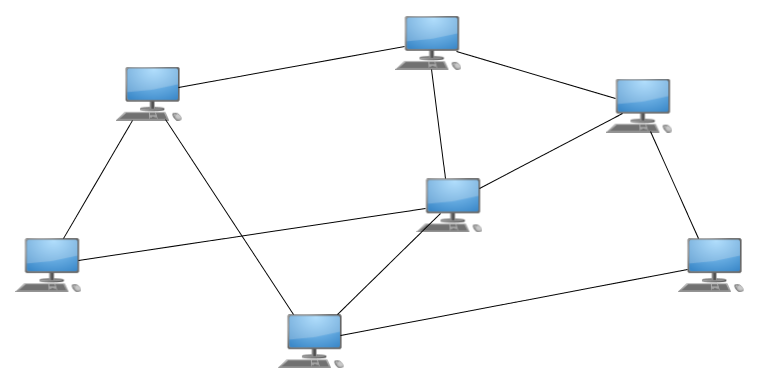
\includegraphics[width=0.6\textwidth]{bilder/network.png}
	\caption{\label{fig:network}Schematische Darstellunge eines Netzwerks als Graph}
\end{figure}


Teilweise ist auch noch die Gesamtanzahl Teilnehmer in Netzwerk bekannt, häufig ist dies aber aufgrund der Grösse und Dynamik nicht möglich.\\
In verteilten Systemen kann es vorkommen, dass sich die Struktur ändert, sich neue Teilnehmer anmelden oder dass Knoten und Verbindungen sich fehlerhaft verhalten oder ganz ausfallen. Verteilte Algorithmen müssen grundsätzlich auch mit solchen Problemen umgehen können, in diesem Bericht wird aber darauf nicht näher eingegangen.\\
Bei den behandelten Anwendungen wird angenommen, dass sich das Netzwerk zur Laufzeit nicht ändert und dass alle Teilemhmer und Verbindungen ohne Fehler funktionieren.


Ein wichtiger Aspekt des Message-Passings ist die Synchronisation der Prozesse. Es gibt dabei verschiedene Ansätze:

\textbf{Synchrones Modell:}
Beim synchronen Modell geht man davon aus, dass bei jedem Prozessor ein interner Timer läuft. Die Timer laufen alle genau gleich schnell und die Prozessoren benötigen für die gleiche Aufgabe die gleiche Zeit. Ausserdem wird angenommen, dass das Versenden von Nachrichten immer die gleiche Zeit dauert, egal über welche Verbindung dies geschieht.

\textbf{Asynchrones Modell:}
In asynchronen Modellen gibt es keinen einheitlichen Takt unter den Prozessoren. Man muss annehmen, dass die Knoten unterschiedlich schnell arbeiten. Um trotzdem verteilte Algorithmen einsetzten zu können, wird bei jedem Knoten eine Queue eingeführt, mit welcher ankommende Nachrichten zwischengespeichert werden.

\begin{figure}[H]
	\centering
		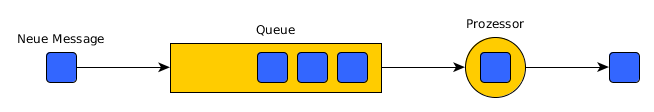
\includegraphics[width=0.6\textwidth]{bilder/queue.png}
	\caption{\label{fig:network}Prozessor mit first-in-first-out Queue}
\end{figure}


Die meisten Netzwerke in der Praxis orientieren sich eher am asynchronen Modell. Gewisse Aspekte aus dem synchronen Modell, wie zum Beispiel ein Timeout falls die Übertragung zu lange dauert, sind jedoch auch häufig anzutreffen. Netzwerkalgorithmen für synchrone Netzwerke können meistens für das asynchrone Modell erweitert werden. Ein Algorithmus, der für ein asynchrones Netzwerk funktioniert, läuft mit Sicherheit auch bei in einen synchronen Netz.


\section{Einheiten für die Komplexität der Algorithmen}
Bei normalen, sequenziellen Algorithmen sind für die Ermittlung der Komplexität meistens die Laufzeit und der benötigte Speicherplatz relevant. Bei verteilten Systemen reichen diese Kriterien nicht mehr aus, um einen Algorithmus beurteilen zu können.
Folgende Kennwerten spielen eine Rolle:

\begin{itemize}
\item \textbf{Anzahl Berechnungsrunden (Computational Rounds)}\\
Die Algorithmen kommen nach einer gewissen Anzahl Berechnungsrunden zum Ergebnis. Bei synchronen Algorithmen kann man die Anzahl Ticks der Timer als Messgrösse benutzen. Im asynchronen Modell laufen die Algorithmen häufig in Wellen von Events durch das Netz. Hier kann somit die Anzahl Wellen eine relevante Grösse sein.

\item \textbf{Benötigter Speicherplatz}\\
Es gibt zwei Kenngrössen für den benötigen Speicher des Algorithmus. Zum einen kann der lokale Speicherplatz auf einem Knoten eine wichtige Information sein. Zum anderen kann über das ganze Netz die Gesamtsumme des benötigten Speichers ausgewertet werden.

\item \textbf{Lokale Laufzeit}\\
Die lokale Laufzeit der Algorithmen auf den Knoten ist auch in verteilten System noch eine wichtige Grösse. Es kann vorkommen, dass die Knoten unterschiedliche Laufzeiten haben, da z. Bsp. Knoten am Rand des Netzes spezielle Aufgaben übernehmen müssen.

\item \textbf{Anzahl und Grösse der Messages}\\
Typischerweise wird analysiert, wie viele Messages für die Ausführung einer Berechnungsrunde versendet werden müssen. Bei Algorithmen mit unterschiedlichen Messagetypen ist auch die Grösse der unterschiedlichen Messages zu beachten.

\end{itemize}

\newpage

\section{Leader Election Ring}
Ein typisches Beispiel eines Netzwerkalgorithmus ist Leader Election. Die Ausgangslage ist ein Ringnetzwerk, bei dem jeder Knoten über eine Nummer identifizierbar ist.\\
Das Ziel ist nun, den Knoten mit der höchsten (oder tiefsten) Nummer zu finden und diese Information im gesamten Ring bekannt zu geben. Somit sollen sich alle Knoten einig sein, welcher als Leader gewählt wurde.\\
Die Knoten kennen lediglich ihre Nummer und den nächsten Knoten, and den sie als einziges Messages senden können.

\begin{figure}[h]
	\centering
		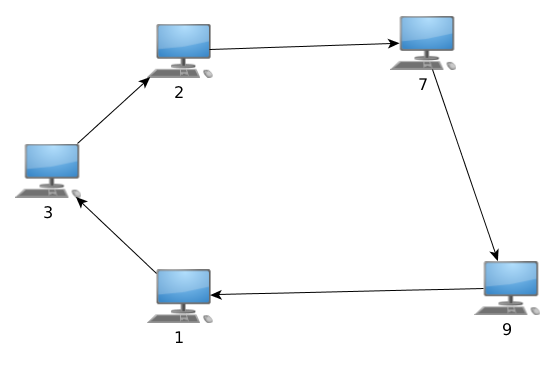
\includegraphics[width=0.5\textwidth]{bilder/ring.png}
	\caption{\label{fig:network}Ausgangslage Leader Election Ring}
\end{figure}

Die Lösung dieses Problems funktioniert nach folgendem Ansatz:

\begin{enumerate}
  	\item Jeder Knoten sendet seine Nummer zum nächsten Knoten
 	\item Wenn eine Nummer empfangen wurde, wird diese mit der eigenen Nummer verglichen
 	\begin{enumerate}
		\item Die grössere der beiden Nummern wird weitergeschickt
        \item Falls die empfangene Nummer die eigenen Nummer ist, ist der Leader gefunden worden
	\end{enumerate}
\end{enumerate}

Es werden zwei verschiedene Messagetypen eingeführt. `Candidate is ...' um einen möglichen Leader dem nächsten Knoten zu melden und `Leader is ...', sobald klar ist, welcher Knoten als Leader bestimmt wurde.
In der ersten Phase werden so lange `Candidate is' Messages versendet, bis die Nummer des Leaders den gesamten Ring durchlaufen hat. Sobald die Message den Ursprungsknoten erreicht hat, wird begonnen `Leader is' Messages zu versenden um die anderen Knoten zu informieren. \\
Dieser Lösungsansatz setzt voraus, dass die Nummern der Knoten eindeutig sind. 

\newpage

\lstset{style=pseudocode}
\begin{lstlisting}[caption=Pseudocode Asynchrone Leader Election in einen Ring Netzwerk]
send Message [Candidate is myId]

finished = false
while not finished
    M = Get Next Message from incoming Queue
    if M is "Candidate is ..." Message then
        if M.id = myId them
            send Message [Leader is myId]
            finished = true
        else
            send Message [Candidate is max(M.id, myId)]
    else
        send M
        finished = true
\end{lstlisting}

Eine Implementation des obigen Algorithmus in Java ist in Anhang \ref{chap:app_leaderElection} zu finden.

Bei einem Ring mit n Knoten sendet in der ersten Phase jeder Knoten n 'Candidate is' Messages. Somit werden in der ersten Phase $O(n^{2})$ Messages versendet.\\
Sobald der Leader bestimmt ist, muss die `Leader is' Message eine komplette Runde durch den Ring absolvieren. In dieser Zeit senden die anderen Knoten weiter `Candidate is' Messages, bis die `Leader is' Message sie erreicht hat. Durchschnittlich versendet jeder Knoten noch \( \frac{n}{2} \) `Candidate is' Messages. Die Message Komplexität des Ring Leader Election Algorithmus entspricht also $O(n^{2})$.



\section{Leader Election Tree} \label{sec_leaderElectionTree}
Für ein Netzwerk das eine Baumstuktur hat, muss der Leader Election Algorithmus natürlich angepasst werden. Der Algorithmus läuft in zwei Phasen ab.
\begin{enumerate}
	\item Die \textbf{Akkumulationsphase} startet bei den externen Knoten (Knoten mit nur einem Nachbarn). Diese senden ihre Nummer an den Nachbar. Jeder Knoten wartet und speichert die eingehenden Nachrichten, bis er von allen ausser einem Nachbarn eine Nachricht erhalten hat. Dann wird die grösste bekannte Nummer an den verbleibenden Knoten gesendet. Sobald ein Knoten von allen Nachbarn Nachrichten erhalten hat, ist der gesamte Baum durchlaufen worden und der verbleibende Knoten kann entscheiden, welcher Teilnehmer als Leader gewählt wird.
    
\begin{figure}[H]
	\centering
		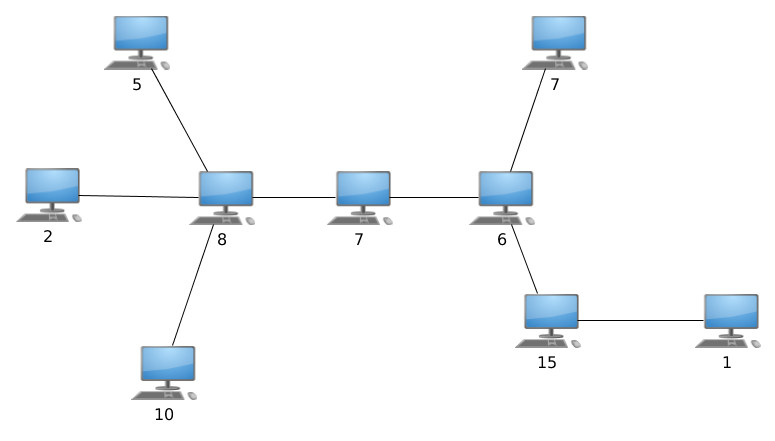
\includegraphics[width=0.6\textwidth]{bilder/leaderElectionTree_1.png}
	\caption{\label{fig:treeLeader_1}Leader Election Tree Ausgangslage}
\end{figure}

\begin{figure}[H]
	\centering
		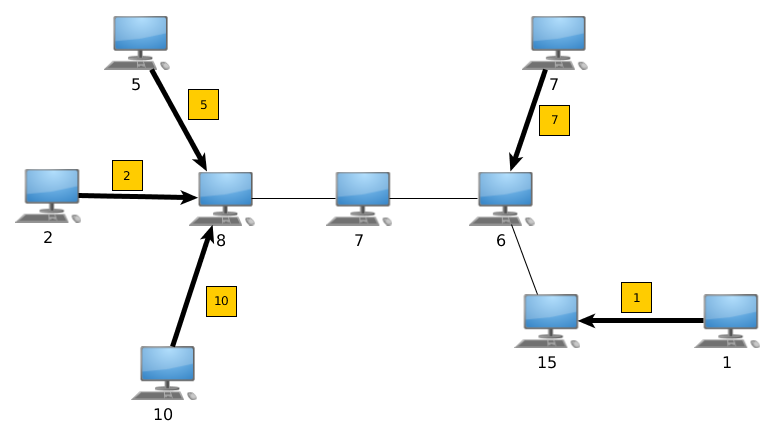
\includegraphics[width=0.6\textwidth]{bilder/leaderElectionTree_2.png}
	\caption{\label{fig:treeLeader_2}Leader Election Tree Accumulation Schritt 1}
\end{figure}

\begin{figure}[H]
	\centering
		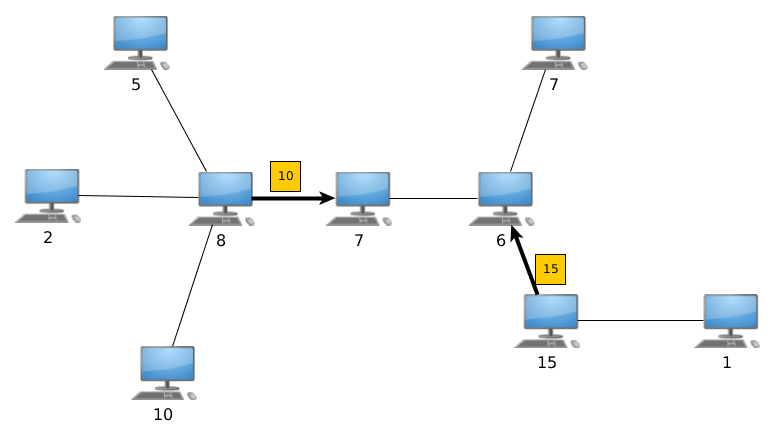
\includegraphics[width=0.6\textwidth]{bilder/leaderElectionTree_3.png}
	\caption{\label{fig:treeLeader_3}Leader Election Tree Accumulation Schritt 2}
\end{figure}

\begin{figure}[H]
	\centering
		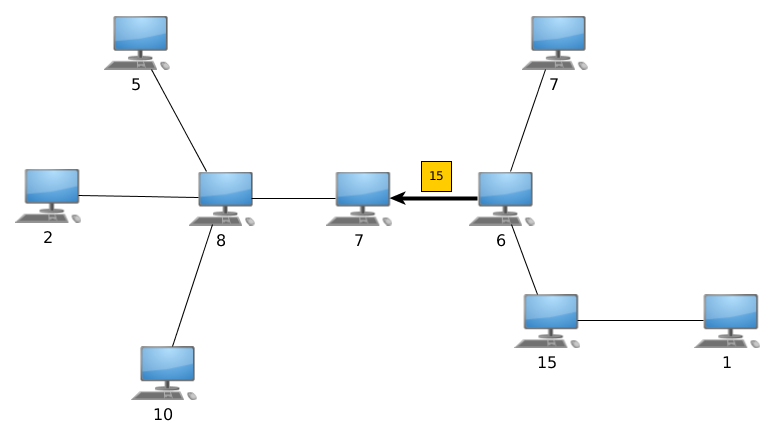
\includegraphics[width=0.6\textwidth]{bilder/leaderElectionTree_4.png}
	\caption{\label{fig:treeLeader_4}Leader Election Tree Accumulation Schritt 3}
\end{figure}
    
    \item Der letzte Node startet nun die \textbf{Broadcastphase}, bei der die Leader Information an jeweils alle Knoten gesendet wird (ausgenonnen vom Nachbarn, von dem die Broadcast Nachricht erhalten wurde).

\begin{figure}[H]
	\centering
		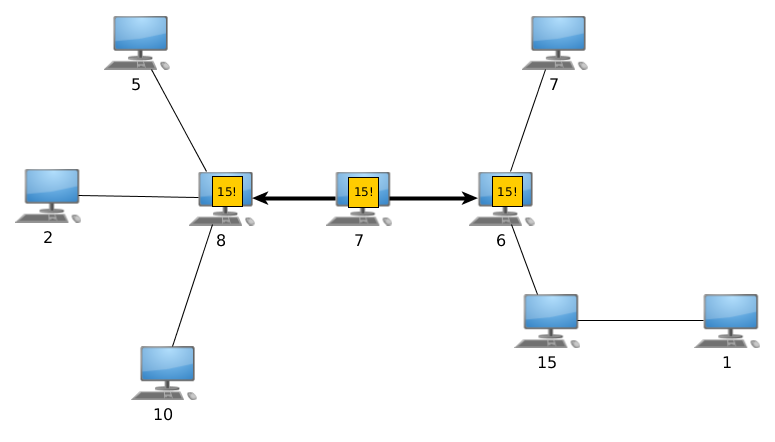
\includegraphics[width=0.6\textwidth]{bilder/leaderElectionTree_5.png}
	\caption{\label{fig:treeLeader_5}Leader Election Tree Broadcast Schritt 1}
\end{figure}

\begin{figure}[H]
	\centering
		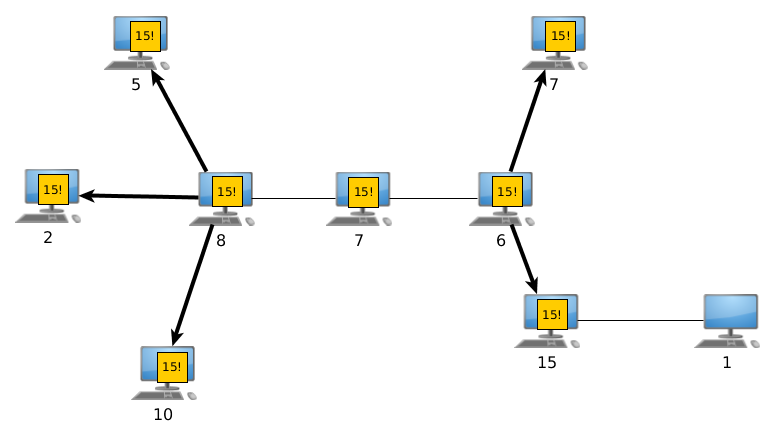
\includegraphics[width=0.6\textwidth]{bilder/leaderElectionTree_6.png}
	\caption{\label{fig:treeLeader_6}Leader Election Tree Broadcast Schritt 2}
\end{figure}

\begin{figure}[H]
	\centering
		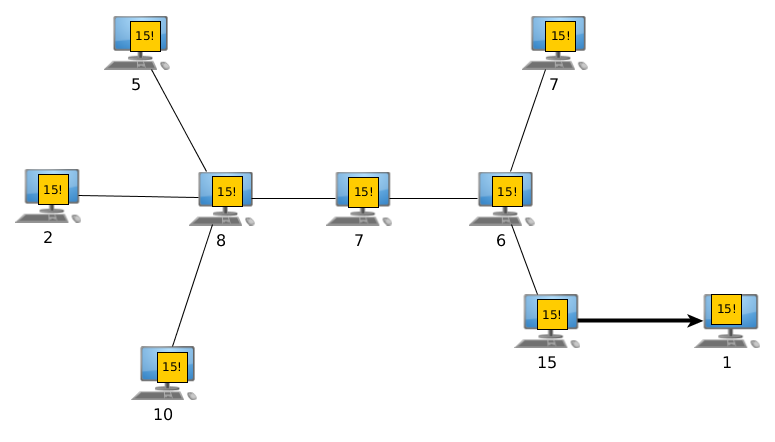
\includegraphics[width=0.6\textwidth]{bilder/leaderElectionTree_7.png}
	\caption{\label{fig:treeLeader_7}Leader Election Tree Broadcast Schritt 3}
\end{figure}

\end{enumerate}

Bei der asynchronen Variante dieses Algorithmus sendet während der Akkumulationsphase jeder Knoten genau eine 'Candidate is'  Nachricht. Für den Broadcast wird schlussendlich an jeden Knoten eine 'Leader is' Message versendet. Die Messages haben eine Grösse von $O(1)$. Somit ist die Message Komplexität bei einem Baum mit n Knoten $O(n)$.


Ein Beispiel für eine praktische Anwendung von Leader Election ist der Clusterverbund von mehreren Servern. Dabei muss ein Server als Leader ermittelt werden, von dem dann koordinative Aufgaben wie Deployment und Logging übernommen werden.



\section{Minimum Spanning Trees}
Der Minimum Spanning Tree eines Graphen ist ein Subgraph, der alle Knoten erreicht und dessen summiertes Gewicht der Kanten minimal ist \cite{wiki:mst}.

\begin{figure}[H]
	\centering
		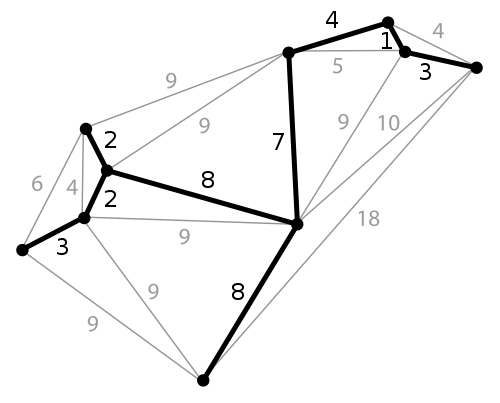
\includegraphics[width=0.5\textwidth]{bilder/500px-Minimum_spanning_tree.png}
	\caption{\label{fig:mst}Beispiel eines Minimum Spanning Trees \cite{wiki:mst}}
\end{figure}

Eine effiziente sequenzielle Lösung für das finden des Minimum Spanning Trees ist der Algorithmus von Baruvka \cite{wiki:boruvka}. Die Idee dabei ist, von jedem Knoten ausgehend Cluster mit dem Nachbarn zu bilden, der über die Kante mit dem kleinsten Gewicht verbunden ist. Der am Schluss entstandenen Graph ist der Minimum Spanning Tree.

Um in verteilten Systemen zu funktionieren, muss der Algorithus angepasst werden. Nachfolged ist die synchrone, verteilte Variante der Minimum Spanning Tree Generierung beschrieben.


\begin{enumerate}
	\item Da die einzelnen Knoten nur ihre direkten Nachbarn kennen, müssen mit Hilfe des Tree Leader Election Algorithmus (siehe Kapitel \ref{sec_leaderElectionTree}) die zusammenhängenden Komponenten bestimmt werden.
    \item Zu jeder zusammenhängenden Komponente muss die Kante gefunden werden mit dem tiefsten Gewicht, die einen neuen Knoten mit der zusammenhängenden Komponente verbindet. Auf jedem Knoten wird nun erneut eine Leader Election durchgeführt, nun mit den angrenzenden Kanten respektiv deren Gewicht.
    \item Dies läuft so lange, bis alle Knoten erschlossen wurden.
\end{enumerate}

In einem Graphen mit n Knoten und m Kanten werden pro Runde $O(m)$ Messsages versendet. Die Anzahl zusammenhängender Komponenten im Graphen halbiert sich mit jeder Runde. Somit gibt es $O(\log{}n)$ Runden, bis der Spanning Tree gefunden wurde. Dies ergibt eine Message Komplexität von $O(m\log{}n)$.

Minimum Spanning Trees werden beispielsweise verwendet, um in einem Netzwerk möglichst effizient eine Nachricht an alle Teilnehmer zu versenden (Broadcast).
